\documentclass[12pt]{article}

% ---- Includerer eksterne filer ------------------------------
\newcommand{\institution}{Forsvarets Høgskole}
\newcommand{\school}{Cyberingeniørskolen Ving 78}
\newcommand{\coursecode}{Matematiske Metoder 2 \\[1ex] ING2501}
\newcommand{\submissiondate}{\today}
\newcommand{\documenttitle}{Bølgeligningen}
\newcommand{\documentsubtitle}{Prosjekt 1}
\newcommand{\authornames}{Morten K. Tverberg \& Mathias Skåret \& Henrik A. Tømt \& Øyvind M. Solend}
\newcommand{\customauthors}{Morten K. Tverberg \\[1ex] Mathias Skåret \\[1ex] Henrik A. Tømt \\[1.5ex] Øyvind M. Solend}
% --- Fjerne unødvendige warnings ---
\usepackage{silence}

% --- Font- og inndatakoding ---
\usepackage[T1]{fontenc}                                % Europeisk fontkoding (korrekte æ/ø/å i PDF)
\usepackage[utf8]{inputenc}                             % Inndata-koding (utf8) for pdflatex


% --- Matematikk (unngå redef-kollisjoner) ---
\usepackage{amsmath}                                    % Bedre matemodus, align/multline/gather
\usepackage{amssymb}                                    % Ekstra matematiske symboler
\usepackage{amsthm}                                     % Teorem-, lemma- og bevis-miljøer
\usepackage{mathtools}                                  % Utvidelser til amsmath (f.eks. \coloneqq)
\usepackage{bm}                                         % Fete greske bokstaver (\bm)

% --- Skrifter, mikrotypografi, bilder ---
\usepackage{newtxtext}                                  % Times-lignende brødtekst
\usepackage[nopatch=footnote]{microtype}                % Mikrosperring/kerning for penere avsnitt
\usepackage{graphicx}                                   % Inkludere bilder (\includegraphics)

% --- Struktur og lister ---
\usepackage{titlesec}                                   % Tilpasse seksjonsoverskrifter
\usepackage{enumitem}                                   % Kontroll på listeinnrykk/spacing

% --- Lenker og referanser ---
\usepackage[unicode]{hyperref}                          % Klikkbare lenker/refs i PDF, metadata

% --- Sideoppsett og enheter ---
\usepackage[a4paper,margin=2.5cm]{geometry}             % Sidestørrelse og marger
\usepackage{siunitx}                                    % SI-enheter og tallformatering (\SI, \num)
\usepackage{setspace}                                   % Justere linjeavstand (\setstretch)

% --- Innholdsfortegnelse og fysikknotasjon ---
\usepackage{tocloft}                                    % Finjustere innholdsfortegnelsen
\usepackage{physics}                                    % Vanlige fysikkmakroer (\dv, \qty, …)

% --- Litteratur ---
\usepackage{csquotes}                                   % Korrekte sitater (anbefalt for biblatex)%
\usepackage[backend=biber,style=ieee]{biblatex}         % Kildehåndtering m/IEEE-stil



% --- Språk ---
\usepackage[main=norsk,english]{babel}              % Orddeling/språk (norsk hovedspråk)

% --- Grafer ---
\usepackage{tikz}                                       % Tegne grafer / piler osv.
\usepackage{pgfplots}                                   % Plotte grafer 
\usetikzlibrary{arrows.meta,calc,angles,quotes}
\pgfplotsset{compat=1.18}
\usepackage{tkz-euclide}

% --- Kode ---
\usepackage{listings}                                   % Inkludere kode med syntax highlighting
\usepackage{xcolor}

% --- Objektorientering i dokumentet ---
\usepackage{float}                                      % Bedre kontroll over plassering av figurer/tabeller
\addbibresource{referanser.bib}
\newcommand{\makedoctitle}{%
  \thispagestyle{empty}
  \begin{minipage}{0.15\textwidth}
      
\includegraphics[height=3cm]{figurer/cisk.png}
  \end{minipage}%
  \begin{minipage}{0.5\textwidth}
      \vspace{10ex}
      {\itshape \institution}\\
      {\bfseries \school}
  \end{minipage}% 
  \begin{minipage}{0.3\textwidth}
      \vspace{13ex}
      \raggedleft
      \today 
  \end{minipage}\\[0.5ex]
  {\rule{\textwidth}{2pt}} \\ \vspace{3ex}

  \begin{center}
      {\fontsize{50}{20}\selectfont \bfseries Prosjektoppgave} \\[1ex]
      {\Large \bfseries \coursecode} \\[10ex]

      {\rule{0.75\textwidth}{0.05pt}} \\[10ex]

      {\fontsize{40}{20}\selectfont \bfseries \documenttitle} \\[10ex]

      {\rule{0.75\textwidth}{0.05pt}} \\[10ex]

      {\huge \bfseries Forfattere:} \\[1ex]
      {\Large \customauthors} \\[1ex]
  \end{center}


\clearpage
}
% ---------------- Dempe unødvendige advarsler  ---------------------------------------
\WarningFilter{latex}{Command \showhyphens has changed}

% ----------------------- Formatering ---------------------------------------
% --- Avsnitt ---
\setlength{\parindent}{0pt}                                                               % Ingen innrykk på første linje i avsnitt
\setlength{\parskip}{0.6\baselineskip plus 2pt minus 1pt}                                 % Dynamisk luft mellom avsnitt (kan strekkes/krympes)

% --- Linjeavstand (litt løsere) --- 
\setstretch{1.10}                                                                         % Litt løsere linjeavstand (typisk 1.10–1.15)

% --- Luft rundt display-matte (equation/align/...) ---
\makeatletter                                                                             
\g@addto@macro\normalsize{%                                                               % Justér standard-verdier for normalsize
  \setlength\abovedisplayskip{-0.3\baselineskip plus 1pt minus 1pt}                        % Luft over display-likninger
  \setlength\belowdisplayskip{1.3\baselineskip plus 1pt minus 1pt}                        % Luft under display-likninger
  \setlength\abovedisplayshortskip{-0.3\baselineskip plus 1pt minus 1pt}                   % Når linja er “kort” før display
  \setlength\belowdisplayshortskip{1.3\baselineskip plus 1pt minus 1pt}                   % Tilsvarende under
}
\makeatother                                                                             

% --- Seksjonsavstand (med titlesec) ---
\titlespacing*{\section}
  {0pt}{2\baselineskip plus .4\baselineskip minus .2\baselineskip}{0.2\baselineskip}    % Venstreinnrykk, før- og etter-avstand
\titlespacing*{\subsection}
  {0pt}{1.1\baselineskip plus .3\baselineskip minus .2\baselineskip}{0\baselineskip}    % Litt strammere for subsection

% --- Lister (med enumitem) ---
\setlist{itemsep=0.4\baselineskip plus 2pt minus 1pt, topsep=0.5\baselineskip}   

% --- Innholdsfortegnelse (med tocloft) ---
\setlength{\cftbeforesecskip}{0.25\baselineskip}                                          % Luft før hver section-linje i ToC
\setlength{\cftbeforesubsecskip}{-0.15\baselineskip}                                      % Luft før hver subsection-linje i ToC

%------------------------Pakke-konflikt-----------------------------
% siunitx vs physics: bruk siunitx sin \qty
\AtBeginDocument{\RenewCommandCopy\qty\SI}
\ExplSyntaxOn
\msg_redirect_name:nnn { siunitx } { physics-pkg } { none }
\ExplSyntaxOff

\emergencystretch=1em

\pgfplotsset{compat=1.18}

                   
% -------------- Stil ------------------------------------------------
\hypersetup{
  colorlinks=true,
  linkcolor=black,
  urlcolor=black,
  citecolor=black,
  pdfauthor={\authornames},
  pdftitle={\documenttitle}
}

\addto\captionsnorsk{%
  \renewcommand{\contentsname}{Innholdsfortegnelse}%      Endrer "Innhold" til "Innholdsfortegnelse"
}

% \DefineBibliographyStrings{norsk}{
%   references = {Kildehenvisninger},                     Kan legges inn hvis ønskelig for å gjøre "Referanser" om til "Kildehenvisninger"
% }

\titleformat{\section}{\large\bfseries}{\thesection.}{0.5em}{}
\titleformat{\subsection}{\normalsize\bfseries}{\thesubsection}{0.5em}{}
\titleformat{\subsubsection}{\normalsize\itshape}{\thesubsubsection}{0.5em}{}


% --------------- Dokument -----------------------------
\begin{document}

\makedoctitle

\pagenumbering{Roman}
\setcounter{page}{1}

\tableofcontents

\clearpage
\addcontentsline{toc}{section}{Sammendrag}
\section*{Sammendrag}
\subsection*{}
\subsubsection*{}
\dots

\subsubsection*{}
\dots


\clearpage

\pagenumbering{arabic}          % Bytter til vanlige tall fra romertall
\setcounter{page}{1}

% ! FJERN FØR INNLEVERING ! ------------------------------
\section*{\color{red}Greit å vite (Fjernes før innlevering)}
1. Kildereferanser gjøres slik: \texttt{\string\parencite\{StringVibration2025\}}, 
se fil referanser.bib for kilder.

2. Hvis du skal legge inn inline-matte i overskrifter/underoverskrifter,
må du bruke \\ \texttt{\string\texorpdfstring\{\$\string\mu\$\}\{mu\}} for eksempelvis $\mu$.

3. 

% ! FJERN FØR INNLEVERING ! ------------------------------

\section{Innledning}
\subsection{Bakgrunn og målsetting}
Bølgeligningen er en av de mest fundamentale partielle differensialligningene i fysikk og matematikk. 
Den beskriver hvordan bølger forplanter seg i tid og rom, og opptrer i mange sammenhenger - fra 
vibrasjoner i en streng eller en membran, til akustiske bølger i luft, seismiske bølger i jordskorpen 
og elektromagnetiske bølger i vakuum. 

I dette prosjektet tar vi utgangspunkt i den klassiske éndimensjonale bølgeligningen:

\begin{equation}
    \frac{\partial^2 u}{\partial t^2} = c^2 \frac{\partial^2 u}{\partial x^2}
    \label{eq:bølgeligningen}
\end{equation}

der $u(x,t)$ beskriver utslaget til systemet, og $c$ er bølgefarten bestemt av materialparametere. 
Vi viser hvordan ligningen kan utledes fra enkle fysiske prinsipper, og hvordan ulike rand- og 
initialbetingelser gir opphav til stående bølger og egenfrekvenser. 

Videre undersøker vi hvordan løsningen oppfører seg under forskjellige forhold, blant annet hvordan 
resonans oppstår når en streng utsettes for en periodisk ytre kraft, og hvordan energien i systemet 
utvikler seg med eller uten demping. Resultatene vil bli både analytisk utledet og numerisk simulert, 
og vi vil sammenligne teori med numeriske observasjoner. 

Formålet med rapporten er dermed å belyse bølgeligningens matematiske struktur, demonstrere sentrale 
fysiske fenomener knyttet til bølger, og trekke paralleller til praktiske anvendelser. Rapporten er 
bygd opp slik at vi først presenterer den teoretiske bakgrunnen og utledningen, deretter beskriver vi 
numeriske metoder og simuleringer, før vi avslutter med resultater, diskusjon og konklusjon.

\subsection{Problemstilling og valg av tema}

I denne oppgaven har vi valgt å fokusere på gitarstrengen som et konkret eksempel på
bølgeligningen i praksis. Problemstillingen vi ønsker å undersøke er:

\begin{center}
    \textit{Hvordan kan strengens materiale, tykkelse og spennkraft modelleres i bølgeligningen, 
    og hvilken betydning har disse faktorene for bølgefarten og dermed tonehøyden på en gitar?}
\end{center}

Vi valgte denne problemstillingen fordi den kombinerer en fundamental matematisk modell 
med et fysisk og praktisk fenomen som de fleste kan relatere til. En gitarstreng er et lettfattelig
eksempel på hvordan bølger oppfører seg, og hvordan små endringer i fysiske parametere kan gi 
merkbare utslag i lyd og tonehøyde. Dermed får vi muligheten til både å fordype oss i 
den matematiske utledningen og samtidig knytte teorien til en konkret anvendelse i musikk.

Problemstillingen er interessant fordi den viser hvordan en enkel partielle differensialligning 
kan forklare komplekse og observerbare fenomener. Samtidig åpner den for en kombinasjon 
av analytiske utledninger og numeriske simuleringer, noe som gir oss mulighet til å sammenligne 
teori og praksis på en strukturert måte.

\subsubsection*{Hvordan vi skal gå frem}

Vi starter med den klassiske bølgeligningen, som beskriver utslaget $u(x,t)$ til en streng i rotnormal retning:

\begin{equation*}
  \frac{\partial^2 u}{\partial t^2} = c^2 \frac{\partial^2 u}{\partial x^2}
  \label{eq:bolgeligningen}
\end{equation*}

og viser hvordan denne kan utledes fra Newtons 2.~lov anvendt på et lite strengsegment.
Videre kobler vi bølgefarten $c$ til strengens fysiske parametere gjennom

\begin{equation}
  c^2 = \frac{T}{\mu}, \qquad \mu \approx \rho 
\end{equation}

der $T$ er spennkraften i strengen, $\rho$ er materialets tetthet og $A$ er strengens tverrsnittsareal.
Som en løsning på bølgeligningen kan vi anta en harmonisk bølge av formen

\begin{equation*}
  u(x,t) = A \sin(kx - \omega t)
\end{equation*}

der $A$ er amplituden, $k=\tfrac{2\pi}{\lambda}$ er bølgetallet og $\omega = 2\pi f$ er vinkelfrekvensen.  
Sammenhengen mellom $\omega$, $k$ og $c$ følger fra dispersjonsrelasjonen

\begin{equation*}
  \omega = c k
\end{equation*}

For en streng med lengde $L$ og faste ender ($u(0,t)=u(L,t)=0$) finner vi at egenfrekvensene blir

\begin{equation*}
  f_n = \frac{n}{2L}\,c, \qquad n=1,2,3,\dots
\end{equation*}

Dermed kan vi analysere hvordan variasjon i $T$, $\rho$ og $A$ påvirker både grunnfrekvensen og de høyere overtonene.
En vilkårlig strengutslag $u(x,0)$ kan videre uttrykkes som en sum av harmoniske svingninger ved hjelp av Fourier-rekker.
Den generelle løsningen for $u(x,t)$ kan uttrykkes med moduser 
$\sin\!\left(\tfrac{n\pi x}{L}\right)$, der tidsdynamikken for hver modus har formen 

\begin{equation*}
    u(x,t) = \sum_{n=1}^{\infty} \bigl[a_n \cos(\omega_n t) + b_n \sin(\omega_n t)\bigr] 
    \sin\!\left(\tfrac{n\pi x}{L}\right).
\end{equation*}

der koeffisientene $a_n$ og $b_n$ bestemmes av de gitte initialbetingelsene.
Fourier rekken gjør det mulig å beskrive komplekse bølgeformer som en sum av enklere, harmoniske svingninger.  
Denne metoden gjør det mulig å uttrykke en strengs bevegelse som en superposisjon av mange enkeltsvingninger med ulike frekvenser og amplituder.  
Ved å bruke denne representasjonen kan man analysere hvordan ulike fysiske faktorer, som spennkraft og tetthet, påvirker bølgefarten og tonehøyden på strengen \parencite{libretextsWave}



Til slutt vil vi sammenligne de utledede teoretiske uttrykkene med numeriske simuleringer 
av bølgeligningen for representative parametere, for å bekrefte modellens gyldighet og illustrere praktiske effekter.

\subsection{Hvordan kunstig intelligens er brukt i arbeidet med rapporten}
I arbeidet med denne oppgaven har vi brukt kunstig intelligens som et supplement, hovedsakelig for å hjelpe med formatering, strukturering og oppsett i LaTeX. 
Selve de matematiske utledningene og formlene har vi gjort på egen hånd, ofte først på papir, før vi har satt dem inn i rapporten. 
Kunstig intelligens har derfor fungert som en støttespiller for å gjøre teksten mer oversiktlig og effektiv å presentere, men den faglige forståelsen, beregningene og drøftingene har vi selv stått for. 
På denne måten har vi sikret at oppgaven gjenspeiler vår egen innsats og kunnskap, samtidig som vi har brukt verktøyet til å styrke klarheten og kvaliteten på framstillingen.

\section{Teori}
\subsection{Fysiske størrelser}

\subsubsection{\texorpdfstring{$u(x,t)$}{u(x,t)}}
$u(x,t)$ beskriver utslaget eller forskyvningen til bølgen i et punkt $x$ til et tidspunkt $t$. 
For en streng representerer dette hvor langt strengen beveger seg i vertikal retning fra likevektsposisjonen.

\subsubsection{Tid \texorpdfstring{$t$}{t}}
Tiden $t$ angir øyeblikket vi observerer bølgen på. 
Den er en kontinuerlig variabel som bestemmer hvordan bølgen utvikler seg.

\subsubsection{Romkoordinatet \texorpdfstring{$x$}{x}}
Koordinatet $x$ beskriver posisjonen langs mediet der bølgen brer seg, for eksempel langs en streng. 
Det gjør at vi kan bestemme bølgens form på forskjellige steder til et gitt tidspunkt.

\subsubsection{Bølgefarten \texorpdfstring{$c$}{c}}
Bølgefarten $c$ forteller hvor raskt bølgeforstyrrelsen brer seg gjennom mediet. 
Høyere bølgefart betyr at forstyrrelser forplanter seg raskere. 
Bølgefarten bestemmes av mediets egenskaper, blant annet strekkspenning og masse per lengdeenhet.

\subsubsection{Strekkraft \texorpdfstring{$T$}{T}}
Strekkraften $T$ beskriver kraften som strengen er strammet med. 
Jo større strekkraft, desto høyere blir bølgefarten i strengen, siden den leder vibrasjoner mer effektivt.
På engelsk omtales dette som \emph{tension}, og defineres som en kraft langs lengden av et fleksibelt medium, 
slik som en streng. \parencite{libretextsTension}

\subsubsection{Masse per lengde \texorpdfstring{$\mu$}{mu}}
$\mu$ er massen fordelt per lengdeenhet av strengen. 
En større $\mu$ betyr at strengen er tyngre, og bølgefarten blir dermed lavere.

\subsection{Utledning av bølgeligningen}
\subsubsection{Krefter på en strengbit, newtons 2.lov}
\dots

\subsubsection{Trinnvis gjennomgang av utledningen}
\dots


\section{Metode}
%\subsection{Utledning av bølgeligningen}
\subsubsection{Forhåndsbetingelser}
For å finne frem til bølgeligningen må man analysere systemet som likningen skal brukes på.
På en gitarstreng er lengden justerbar, men tonen endres primært ved å stramme eller slakke
strengen.

En gitarstreng modelleres som en tråd som er spent mellom to punkter, der den er fiksert på plass.
I normaltilstand ligger strengen stram i en rett linje mellom punktene, frem til den plukkes. Da
forstyrres likevekten, og strengen begynner å vibrere. Problemet er da å finne en $u(x,t)$ som modellerer
defleksjonen til strengen. Hvis strengen har lengde $l$, massetetthet $\rho$ og slippes ved $t=0$,
vil modellen beskrive defleksjonen $u(x,t)$ for vilkårlig $x$ når $t>0$.

Forutsetninger for løsning av bølgeligningen:

\begin{enumerate}
  \item Gravitasjon er neglisjerbar i forhold til strengspenningen.
  \item Alle defleksjoner er små og skjer i samme plan.
  \item Massen per lengde er konstant over hele strengen, slik at spenningen er den samme
  gjennom hele strengen.
\end{enumerate}
\clearpage
\subsubsection{Utledning}

\begin{figure}[H]
  \centering
  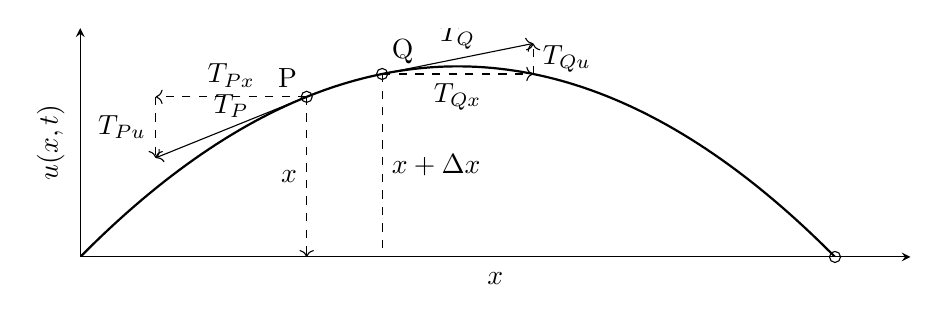
\begin{tikzpicture}
    \begin{axis}[
      width=\textwidth,
      height=0.37\textwidth,
      axis lines=left,
      xlabel={$x$},
      ylabel={$u(x,t)$},
      xmin=0, xmax=1.1,
      ymin=0, ymax=0.6,
      xtick=\empty,
      ytick=\empty
    ]

      % punkter
      \coordinate (Ppoint)  at (axis cs:0.3,0.42);
      \coordinate (Pupoint) at (axis cs:0.1,0.26);
      \coordinate (Pxpoint) at (axis cs:0.1,0.42);
      \coordinate (Qpoint)  at (axis cs:0.4,0.48);
      \coordinate (Qupoint) at (axis cs:0.6,0.56);
      \coordinate (Qxpoint) at (axis cs:0.6,0.48);

      % strengkurve
      \addplot[domain=0:1, samples=100, thick] {-2*x^2 + 2*x};

      % krefter ved P
      \draw[->, thin] (Ppoint) -- (Pupoint) node[midway, above] {$T_P$};
      \draw[->, thin, dashed] (Ppoint) -- (Pxpoint) node[midway, above] {$T_{Px}$};
      \draw[->, thin, dashed] (Pxpoint) -- (Pupoint) node[midway, left]  {$T_{Pu}$};

      % krefter ved Q
      \draw[->, thin] (Qpoint) -- (Qupoint) node[midway, above] {$T_Q$};
      \draw[->, thin, dashed] (Qpoint) -- (Qxpoint) node[midway, below] {$T_{Qx}$};
      \draw[->, thin, dashed] (Qxpoint) -- (Qupoint) node[midway, right] {$T_{Qu}$};

      % loddrette hjelpelinjer
      \draw[->, dashed] (axis cs:0.3,0.42) -- (axis cs:0.3,0) node[midway, left] {$x$};
      \draw[dashed]     (axis cs:0.4,0.48) -- (axis cs:0.4,0) node[midway, right] {$x+\Delta x$};

      % punktsymboler og etiketter
      \addplot[only marks, mark=o] coordinates {(0.3,0.42) (0.4,0.48) (1,0)};
      \node[anchor=south east] at (Ppoint) {P};
      \node[anchor=south west] at (Qpoint) {Q};
      \node[anchor=north]      at (axis cs:1,0) {$l$};

    \end{axis}
    \end{tikzpicture}
  \caption{Krefter og vinkler på et lite strengstykke $[x,\,x+\Delta x]$.}
\end{figure}

For å finne likningen betraktes et lite stykke av strengen ved $t=0$, med lengde $\Delta x$ og start i
$x$. Punktet $P=(x,u(x,0))$ og punktet $Q=(x+\Delta x, u(x+\Delta x,0))$ er endene av strengstykket.
$T$ er kraften som spenningen i strengen skaper i et punkt $x>0$ langs strengen. 
$\alpha$ er vinkelen mellom $T_{Qx}$ og $T_Q$, og $\beta$ er vinkelen mellom
$T_{Px}$ og $T_P$.

\begin{align*}
  T_{Px} = T_P \cos\beta, &\qquad T_{Qx} = T_Q \cos\alpha,\\
  T_{Pu} = T_P \sin\beta, &\qquad T_{Qu} = T_Q \sin\alpha.
\end{align*}

Fordi spenningen i strengen er lik over hele strengen, vil de horisontale kreftene
av $T_Q$ og $T_P$ utjevne hverandre:

\begin{equation}
  T_{Px} = T_{Qx} = T = \text{const.}
  \label{eq:horisontaleKrefterKonstant}
\end{equation}

Ifølge Newtons andre lov $(F=ma)$ for strengstykket settes massen lik $m=\rho\,\Delta x$ og
akselerasjonen $a=u_{tt}$. Kraften som virker på strengen er $F=T_{Qu}-T_{Pu}$. Da får vi:

\begin{equation*}
  T_{Qu}-T_{Pu}=\rho\,\Delta x\,\frac{\partial^2 u}{\partial t^2}.
\end{equation*}

Videre brukes $\tan\theta=\frac{\sin\theta}{\cos\theta}$ sammen med \eqref{eq:horisontaleKrefterKonstant}, og
$\tan\alpha$ og $\tan\beta$ antas små (små defleksjoner), slik at forenklinger kan benyttes: 

\begin{equation}
  \frac{T_{Qu}}{T_{Qx}}-\frac{T_{Pu}}{T_{Px}}
  = \tan\alpha - \tan\beta
  = \frac{\partial u}{\partial x}(x+\Delta x,t)-\frac{\partial u}{\partial x}(x,t)
  = \frac{\rho\,\Delta x}{T}\,\frac{\partial^2 u}{\partial t^2}.
  \label{eq:krefterPaStykke}
\end{equation}
\clearpage
Ganger man begge sider med $\dfrac{T}{\rho\,\Delta x}$:

\begin{equation}
  \frac{\partial^2 u}{\partial t^2}
  = \frac{T}{\rho\,\Delta x}\left[
     \frac{\partial u}{\partial x}(x+\Delta x,t)-\frac{\partial u}{\partial x}(x,t)
    \right].
  \label{eq:tidPartiellDerivert}
\end{equation}

Setter man $\Delta x\to 0$ som grenseverdi, fremkommer definisjonen av den deriverte:

\begin{equation}
  \frac{\partial^2 u}{\partial t^2}
  = \lim_{\Delta x\to 0}\frac{T}{\rho}\frac{1}{\Delta x}
    \left[\frac{\partial u}{\partial x}(x+\Delta x,t)-\frac{\partial u}{\partial x}(x,t)\right]
  = \frac{T}{\rho}\,\frac{\partial^2 u}{\partial x^2}.
  \label{eq:deltaXGarMotNull}
\end{equation}

Setter man $c^2=\dfrac{T}{\rho}$ får vi bølgeligningen: 

\begin{equation}
  \frac{\partial^2 u}{\partial t^2}
  = c^2\,\frac{\partial^2 u}{\partial x^2},
  \qquad
  c^2=\frac{T}{\rho}.
  \label{eq:utledetBolgelikning}
\end{equation}

\subsection{Metode og verktøy for numerisk løsning}
\subsubsection{Valg av verktøy}
For å løse bølgeligningen numerisk har vi valgt å bruke Python. Språket er mye brukt innen
vitenskapelige beregninger og har et stort økosystem av biblioteker som forenkler implementasjon av
numeriske metoder og visualisering av resultater. Innenfor bibliotekene \texttt{NumPy} og \texttt{Matplotlib}
finnes funksjonalitet som gjør det enkelt å løse oppgaver numerisk og fremstille resultatene grafisk.
Dette gjør Python til et velegnet valg for denne problemstillingen. For animasjoner av resultatene bruker
vi \texttt{matplotlib.animation} (en del av \texttt{Matplotlib}); dette gir en mer intuitiv forståelse av
hvordan løsningen utvikler seg over tid. Til 2D-grafer benyttes \texttt{matplotlib.pyplot}. For å forstå
komplekse ligninger som bølgeligningen er det nyttig å kunne visualisere resultatene på en enkel og
konsis måte.

\subsection{Løsning med separasjon av variable}
\begin{equation}
	u_{tt} = c^2 u_{xx} \qquad \iff \qquad 
	\frac{\partial^2 u}{\partial t^2} = \frac{T}{\rho} \frac{\partial^2 u}{\partial x^2}	
	\label{eq:bølgelikningForLøsning}
\end{equation}

En løsning av bølgeligningen forutsetter definerte rand- og initialbetingelser. Strengen har fast lengde $l$
og er festet i begge ender; dette er randbetingelsene. Initialbetingelsene gjelder ved $t=0$, hvor strengen
slippes fra en posisjon bestemt av $f(x)$. Ettersom strengen slippes, settes $u_t(x,0) = 0$.
\clearpage
Grensebetingelsene for funksjonen $u(x,t)$ blir derfor:

\begin{align}
	u(0 , t) = 0 \label{eq:grensebetingelse0}\\
	u(l , t) = 0 \label{eq:grensebetingelsel}
\end{align}

og initialbetingelsene for funksjonen $u(x,t)$ blir:

\begin{align}
	u(x , 0) &= f(x) = \sum_{n=0}^{n=\infty} c_n \sin \left( \frac{n \pi}{l} x \right) 	
	\label{eq:initialbetingelse1}
\end{align}

Separasjon av variabler går ut på å finne to funksjoner $F(x)$ og $G(t)$ slik at $u(x , t)=F(x)G(t)$.
Da separeres tid $t$ og posisjon $x$ i to ulike funksjoner.

\begin{equation*}
	u(x , t) = F(x)G(t)
\end{equation*}

De partiellderiverte av $F(x)$ og $G(t)$ blir:

\begin{equation}
	u_{tt} = F(x)G''(t), \qquad u_{xx} = F''(x)G(x)
	\label{eq:separasjonPartiellDeriverte}	
\end{equation}

Setter vi \eqref{eq:separasjonPartiellDeriverte} inn i \eqref{eq:bølgelikningForLøsning}:

\begin{align*}
  \hspace{35ex}
  u_{tt} &= c^2 u_{xx} \\
  \hspace{2ex} F(x)G''(t) &= c^2 F''(x)G(t) \hspace{10ex} \vert 
  \cdot \frac{1}{c^2 F''(x) G''(t)} \\
  \frac{F''(x)}{F(x)} &= \frac{1}{c^2} \frac{G''(t)}{G(t)}
\end{align*}

For at begge sider skal være like for alle $x \in \left[ 0 , l \right]$ og $t < 0$ må uttrykket være lik en
konstant. Denne settes til $- \lambda^2$. Den velges negativ for å gi sinus- og cosinusløsninger (ikke
eksponentielle). Med kvadrert parameter sikres positivitet:

\begin{equation*}
	\frac{F''(x)}{F(x)} = \frac{1}{C^2} \frac{G''(t)}{G(t)} = - \lambda^2
\end{equation*}
\clearpage
$F(x)$ og $G(t)$ er dermed to differensiallikninger som kan løses. Med $F(x)$, og
grensebetingelsene (\ref{eq:grensebetingelse0}) og (\ref{eq:grensebetingelsel}) blir første differensialligning mulig å løse:

\begin{align*}
	\hspace{20ex} \frac{F''(x)}{F(x)} &= - \lambda^2 \hspace{10ex} \vert \cdot F(x)\\
	F''(x) + \lambda^2&F(x) = 0
\end{align*}

Løses dette som en 2.\ ordens homogen differensiallikning blir resultatet:

\begin{align*}
	F''(x) + \lambda^2&F(x) = 0 \\ 
	\Rightarrow r^2 + &\lambda^2 = 0 \\
	\Rightarrow r_1 = 0 - i \lambda &\vee r_2 = 0 + i \lambda \\
	\Rightarrow F(x) = e^{0 \cdot x} & \left( \alpha  \cos \lambda x + \beta \sin \lambda x \right) \\
	\Rightarrow F(x) = \alpha \cos& \lambda x + \beta \sin \lambda x 
\end{align*}

Settes grensebetingelse (\ref{eq:grensebetingelse0}) inn:

\begin{align*}
	u(0 , t) = F(&0)G(t) = 0\\
	\Rightarrow F(0) = \alpha \cos&\lambda \cdot 0 + \beta \sin \lambda \cdot 0 \\
	\Rightarrow F(0) = \alpha \cos&0 + \beta \sin 0 \\
	\Rightarrow F(0) = &\alpha = 0 \\
	\Rightarrow \alpha =& 0 \\
	\Rightarrow F(x) = &\beta \sin \lambda x
\end{align*}

Videre brukes grensebetingelse (\ref{eq:grensebetingelsel}) for å finne $\lambda$:

\begin{align*}
	u(l ,t) = F(l&)G(t) = 0 \\
	\Rightarrow F(l) =& 0 \\
	\Rightarrow \beta \sin \lambda &\cdot l = 0 \\ 
	\Rightarrow \lambda = \frac{\pi n}{l}&, \qquad n \in \mathbb{N} \\
	\Rightarrow F(x) = { \beta }_n & \sin \frac{\pi n}{l} x
\end{align*}

Nå er uttrykket for $\lambda$ og $F(x)$ funnet; neste steg er å finne $G(t)$:

\begin{align*}
	G''(t) = - \lambda^2 & c^2 G(t) \\
	\Rightarrow G''(t) + \lambda^2 & c^2 G(t) = 0 
\end{align*}

Dette løses som en 2.\ ordens homogen differensiallikning:

\begin{align*}
	G''(t) + \lambda^2 & c^2 G(t) = 0 \\
	\Rightarrow r^2 + \lambda^2 c^2 = 0 \\
	\Rightarrow r_1 = 0 + i \lambda c &\vee r_2 = 0 - i \lambda c \\ 
	\Rightarrow G(t) = e^{0 t} \gamma&\cos c \lambda t + \psi \sin c \lambda t \\
	\Rightarrow G(t) = \gamma\cos & c \lambda t + \psi \sin c \lambda t
\end{align*}

Ettersom strengen slippes fra startposisjonen bestemt av (\ref{eq:initialbetingelse1}) og startfarten settes til $u_t(x,0)=0$,
blir $\psi=0$, og $G(t)$ reduseres til:

\begin{equation*}
	G(t) = \gamma \cos c \lambda t = \gamma \cos \frac{c \pi n}{l} t
\end{equation*}

Settes sammen $F(x)$ og $G(t)$, blir løsningen:

\begin{equation}
	u(x,t) = \sum_{n=0}^{\infty} c_n 
	\sin \left( \frac{n \pi}{l} x \right)
	\cos \left( \frac{n \pi c}{l} t \right)
	\label{eq:bølgelikningLøst}	
\end{equation}

\subsubsection{Konstanten \texorpdfstring{$c_n$}{cn}}

Konstanten $c_n$ beskriver initialbetingelsene. For en streng med lengde
$l$ og initialform $f(x)$ (slik at $u(x,0)=f(x)$) blir:

\begin{equation}
	c_n = \frac{2}{l} \int_{0}^{l} f(x) \sin \left( \frac{n \pi}{l} x \right) \,dx
	\label{eq:cnDefinisjon}
\end{equation}

\subsubsection{Beskrivelse av maple kode}

Maple-koden starter med å definere initialbetingelsene for simuleringen. Strengen er $l = 64{,}77\,\text{cm}$ lang og dras
opp i punkt $x = a = 7\,\text{cm}$ til høyde $u(a,0) = h = 2\,\text{cm}$. For å estimere tettheten til gitarstrenger brukes 
formelen $\rho = 7825\,\text{kg/m}^3 \cdot \pi (0.00256 \cdot \texttt{string\_gauge} /2)^2$. Strengtykkelsene er hentet fra
Ernie Ball Super Slinky \parencite{ErnieBallSlinky}, og $7825\,\text{kg/m}^3$ er massetetthet for stål ifølge Wikipedia \parencite{WikipediaTetthet},
idet det antas at alle strengene er stålstrenger. Ved beregning av strengspenning ble en strengspenningskalkulator brukt
\parencite{RodrigoStringTensionCalc}, med valg «0.009 D'Addario / Ernie Ball». Deretter defineres $f(x)$, $c_n$ og $u(x,t)$,
og \verb|explore| samt \verb|plot| benyttes for å visualisere alle strengene i én graf, der $t$ styres med en glider.
Det var ikke trivielt å legge inn strengenes navn i plottet, noe som gjør det vanskelig å skille kurvene. Under følger en tabell
med strengtykkelser, massetetthet, strengspenning og $c$-verdi. Koden fra maple kan hentes her: \parencite{mapleKode}

\begin{table}[!h]
	\centering
	\begin{tabular}{|c|c|c|c|c|}
		\hline
		Streng & strengtykkelse & massetetthet, $\rho$ & strengspenning, $T$ & $c$-verdienre \\  
		\hline
		E4 & $0.009''$ & $3,26 mg/m$ & $58,49N$ & $4,24 km/s$ \\	
		B3 & $0.011''$ & $4,87 mg/m$ & $47.99N$ & $3,14 km/s$ \\
		G3 & $0.016''$ & $10,3 mg/m$ & $65,29N$ & $2,51 km/s$ \\
		D3 & $0.024''$ & $23,2 mg/m$ & $69,62N$ & $1,61 km/s$ \\
		A2 & $0.032''$ & $41,2 mg/m$ & $70,09N$ & $1,30 km/s$ \\
		E2 & $0.042''$ & $71,0 mg/m$ & $65,06N$ & $1,16 km/s$ \\
		\hline
	\end{tabular}
	\caption{Tabell over gitarstrenger og deres respektive fysiske verdier}
	\label{tab:listeOverGitarstrenger}
\end{table}

\subsection{Beskrivelse av kode for numerisk løsning}
\subsubsection{Pakker, variabler og parametere}
I dette delkapittelet beskrives en numerisk tilnærming til bølgeligningen (koden kan hentes fra 
\parencite{simuleringKode}). 

Først importeres nødvendige pakker for numeriske beregninger og grafisk fremstilling: \texttt{NumPy} for numerikk,
\texttt{matplotlib.pyplot} for plotting og \texttt{matplotlib.animation} for animasjon (jf.\ forrige seksjon).
Deretter settes konfigurasjonsparametere som definerer strengens fysiske egenskaper og parametere for den numeriske 
løsningen. Dette inkluderer lengden $L$, bølgehastigheten $c$ og simulert varighet $s$. Videre defineres antall
punkter $N$ til å dele opp strengen. Dette påvirker nøyaktigheten: flere punkter gir bedre oppløsning, men øker
beregningstid og minnebruk. Antall moduser bestemmer detaljgraden i startformen, der høyere verdi gir skarpere kanter og
mer høyfrekvent innhold. 

Videre settes grafiske parametere, som \texttt{fps} (frames per second) for animasjonen og linjetykkelse. Startformen 
settes med
\begin{lstlisting}
  initial_shape_type = "pluck"
  pluck_width: float = 0.15
\end{lstlisting}
der \verb|"pluck"| angir en plukk (trekant-/teltform), og \verb|pluck_width| definerer bredden på området som plukkes.

\subsubsection{Initialbetingelser-funksjonen}
Hensikten er å definere startformen ved $t=0$, altså å returnere $u(x,0)$.
Funksjonen tar inn en $\verb|x|$-array (posisjoner langs strengen). Avhengig av \verb|initial_shape_type|
returneres ulike startformer. I vårt tilfelle gir \verb|"pluck"| en trekantformet profil, der plukkposisjon og bredde styrer formen:
\begin{lstlisting}
  if initial_shape_type == "pluck":
    center = pluck_position * length_m
    width = pluck_width * length_m
    return np.clip(1.0 - np.abs(x - center) / width, 0.0, 1.0)
\end{lstlisting}

Med verdiene satt i starten av koden får vi figuren under:

\begin{figure}[H]
    \centering
    \begin{tikzpicture}
        \begin{axis}[
        width=0.9\textwidth,
        height=0.5\textwidth,
        axis lines=left,
        xlabel={$x$ [m]},
        ylabel={$u(x,0)$ [m]},
        xmin=0, xmax=1.02,
        ymin=-1.1, ymax=1.1,
        xtick={0.15, 0.45, 1},
        ytick={-1, 0, 1}
        ]
        
        \draw (0,0) -- (0.15,0);
        \draw [dashed] (0.15,0) -- (0.3,1) -- (0.45,0);
        \draw (0.45,0) -- (1,0);
        \fill (0.3,1) circle (2pt);

        \end{axis}
    \end{tikzpicture}
    \caption{Startform ved $t=0$ når strengen plukkes ved $x=0.3$ m.}
\end{figure}

Her ser vi at strengen plukkes i en trekantformet bølge med høyde $y=1.0\,\text{m}$ og bredde $0.15\,\text{m}$.
Dette er ikke en nøyaktig kopi av en fysisk plukk, men en hensiktsmessig tilnærming som er enkel å implementere.

Startfarten settes til null over hele strengen ved $t=0$. Funksjonen $g(x)=u_t(x,0)$ returnerer derfor
\verb|np.zeros_like(x)| (en array med samme form som \verb|x|, men med bare nuller).

\subsubsection{Oppsett av romlige og tidsmessige akser}
Første linje (\verb|np.ndarray x|) oppretter et jevnt fordelt rutenett fra $0$ til lengden $L$. Punktene representerer
posisjoner der $u(x,t)$ evalueres. Som eksempel: med \verb|num_points=5| og \verb|length_m=1.0| blir \verb|x = [0, 0.25, 0.5, 0.75, 1.0]|.
Variabelen \verb|dx| beregnes for informasjon (ikke brukt videre). Deretter settes tidssteget \verb|dt| til $\tfrac{1}{\texttt{fps}}$,
slik at for \verb|fps=60| oppdateres tilstanden hver $\approx 16{,}7$ ms. Antall tidssteg settes med
\verb|num_steps = int(duration_s * fps) + 1|, og \verb|t| blir arrayen med alle tidspunkter der strengen evalueres.

\subsubsection{Metodefunksjonen}
Denne funksjonen starter selve simuleringen. Bevegelsen oppstår fra de definerte initialbetingelsene og beregnes trinnvis over tid:

\begin{equation*}
  u(x,t) = \sum_{n=1}^{N} 
  \big[ B_n \cos(\omega_n t) + B_n^{*} \sin(\omega_n t) \big]
  \sin\!\left(\frac{n\pi x}{L}\right)
\end{equation*}

Først hentes startform \verb|f| og starthastighet \verb|g| fra funksjonene over. Deretter konstrueres en kolonnevektor med
modusindekser, og basisfunksjonene $\sin\!\left(\frac{n \pi x}{L}\right)$ for alle $n$. Resultatet er en matrise med
$N$ (moduser) $\times$ $N_x$ (rompunkter). Egenfrekvensene settes til $\omega_n = c \frac{n \pi}{L}$ for en streng med faste ender.
Fourier-koeffisientene beregnes fra $f$ og $g$ ved

\begin{align*}
  B_n &= \frac{2}{L} \int_{0}^{L} f(x)\,\sin\!\left(\frac{n\pi x}{L}\right)\,dx \\
  B_n^{*} &= \frac{2}{L\,\omega_n} \int_{0}^{L} g(x)\,\sin\!\left(\frac{n\pi x}{L}\right)\,dx
\end{align*}

Deretter allokeres en matrise for alle tidssteg (rader: tid, kolonner: rompunkter $x$). For hvert $t_k$ beregnes de tidsavhengige
koeffisientene, og $\sum_n a_n(t_k) \sin\!\left(\frac{n \pi x}{L}\right)$ utføres vektoriserte med \verb|coeff_t @ sin_basis|:
\begin{lstlisting}
  frames = np.zeros((num_steps, num_points))
  for k, tk in enumerate(t):
      coeff_t = B * np.cos(omega_n * tk) + B_star * np.sin(omega_n * tk)
      frames[k, :] = coeff_t @ sin_basis
\end{lstlisting}

Til slutt håndheves randbetingelsene $u(0, t) = u(L, t) = 0$ numerisk for robusthet (siden \verb|np.trapz|
gir en tilnærming og \verb|num_modes=60| ikke er $\to\infty$). Funksjonen returnerer hele tidsutviklingen $u(x, t_k)$.

\subsubsection{Animasjonsfunksjonen}
Funksjonen tar inn alle simulerte rammer (2D-array \verb|(num_steps, num_points)|) samt en tittel. Det opprettes figur og akse,
før første tidsramme tegnes. X-aksen settes til strengens lengde, y-aksen dimensjoneres fra min./maks.\ verdi med litt
padding. Aksenavn, tittel og en tidslabel oppdateres fortløpende via \verb|update(i)|, mens \verb|init()| tegner startbildet.
Selve animasjonen settes opp med:

\begin{lstlisting}
  anim = FuncAnimation(
    fig,
    update,
    frames=range(0, len(frames), 1),
    init_func=init,
    interval=1000 / (0.25* fps),
    blit=True,
    )
\end{lstlisting}

Avslutningsvis lagres animasjonen lokalt, samt et stillbilde for $t=0$.


\section{Resultater}
\subsection{Teoretiske resultater}
\subsubsection{Uteldning av egenfrekvenser}
For en streng som er festet i to punkter er hastigheten $v$ gitt ved:

\begin{equation*}
    v = \sqrt{\frac{T}{\mu}}
\end{equation*}
Hvor $T$ er spenningen i strengen og $\mu$ er massetettheten. 

Forholdet mellom hastighet ($v$), frekvens ($f$) og bølgelengde ($\lambda$) er gitt ved

\begin{equation*}
    v = f \lambda
\end{equation*}  

Når strengen er festet i begge ender, kan den bare svinge i bestemte mønstre, kalt normalmoduser.
Den enkleste normalmodusen er grunnmodusen, som har en bølgelengde som er dobbelt så lang som strengen:

\begin{equation*}
    \lambda_1 = 2L
\end{equation*}
Hvor $L$ er lengden på strengen.

Frekvensen til grunnmodusen kan dermed uttrykkes som:

\begin{equation*}
    f_1 = \frac{v}{\lambda} = \frac{1}{2L} \sqrt{\frac{T}{\mu}}
\end{equation*}
Dette er Mersenne's likning.




\subsubsection{Normalmoduser}

Det er uendelig mange normalmoduser for en streng som er festet i begge ender.
Som nevnt tidligere er grunnmodusen den enkleste normalmodusen og er den med lavest frekvens.

Hver påfølgende normalmodus har en frekvens som er et helt multiplum av grunnmodusen,
hvor $n$ er et positivt heltall som representerer modustallet.

Dette kan utledes ved å merke seg at for den $n$-te normalmodusen, er bølgelengden gitt ved:

\begin{equation*}
    \lambda_n = \frac{2L}{n}
\end{equation*}
Ved å sette dette inn i bølgeformelen $v = f \lambda$, får vi:

\begin{equation*}
    f_n = \frac{v}{\lambda_n} = \frac{1}{\frac{2L}{n}} \sqrt{\frac{T}{\mu}} = \frac{n}{2L} \sqrt{\frac{T}{\mu}}
\end{equation*}
Dermed er frekvensen til den $n$-te normalmodusen:

\begin{equation*}
    f_n = n f_1 = \frac{n}{2L} \sqrt{\frac{T}{\mu}}
\end{equation*}
Hvor $n = 1, 2, 3, \ldots$.




\subsection{Numeriske resultater}
\subsubsection{Visualisering av strengens bevegelse}
\begin{figure}[h!]
\centering
\begin{tikzpicture}[scale=1.0]
  % aksene
  \draw[->] (-0.5,0) -- (11,0) node[right] {$x$};
  \draw[->] (0,-2.5) -- (0,2.5) node[above] {$y$};

  % parametre
  \def\A{2} % amplitude
  \def\nodes{0, 5, 10} % noder

  % stående bølge: y = 2*sin(x), snapshot
  \draw[blue, thick, samples=200, domain=0:10] 
        plot (\x, {\A*sin(deg(pi*\x/5))});

  % markere noder
  \foreach \x in \nodes {
    \fill[black] (\x,0) circle (2pt);
  }

  % litt forskjøvet bølge (stiplet)
  \draw[red, thick, dashed, samples=200, domain=0:10] 
        plot (\x, {\A*sin(deg(pi*\x/5))*0.7});
\end{tikzpicture}
\end{figure}




\subsubsection{Sammenligning med teoretiske resultater}
\dots

\subsubsection{Parametervariasjon}
\dots

\section{Diskusjon}
\subsection{Tolkning av resultater}
\subsubsection{Kort oppsummering av funn}
I dette arbeidet er bølgelikningen for en streng utledet både teoretisk og implementert numerisk. Utgangspunktet er en fysisk modell av en streng festet i begge ender, og påvirket av en spenning, der man ved hjelp av Newtons lover og Taylor-utvikling kommer fram til bølgelikningen:

\begin{equation*}
\frac{\partial^2 u}{\partial t^2} = \frac{T}{\rho} \frac{\partial^2 u}{\partial x^2}
\end{equation*}

Her er \( T \) spenningen i strengen, \( \rho \) massetettheten, og \( u(x, t) \) beskriver utslaget til strengen. Bølgehastigheten defineres som

\begin{equation*}
c^2 = \frac{T}{\rho}
\end{equation*}

Den teoretiske løsningen gjøres ved separasjon av variable, hvor løsningen antas å være et produkt av en romlig funksjon \( F(x) \) og en tidsavhengig funksjon \( G(t) \). Dette fører til to separate differensiallikninger, som løses med sinus- og cosinus-funksjoner. Ved å bruke grensebetingelser for en streng som er fast i begge ender, finner man en løsning som uttrykkes som en uendelig sum (Fourier-rekke) av normalmoduser:

\begin{equation*}
u(x, t) = \sum_{n=1}^{\infty} c_n \sin\left(\frac{n\pi x}{l}\right)\cos\left(\frac{n\pi c t}{l}\right)
\end{equation*}

Den numeriske løsningen er implementert i Python, hvor bibliotekene \texttt{NumPy} og \texttt{Matplotlib} benyttes til henholdsvis beregninger og visualisering. Startformen til strengen ved \( t = 0 \) defineres som en trekantform (\textit{pluck}), som er en forenklet, men effektiv modell av hvordan en streng kan plukkes i praksis. Videre brukes \texttt{Matplotlib.animation} for å vise hvordan strengen beveger seg over tid.

Til slutt beregnes de teoretiske egenfrekvensene for strengen. Når strengen er festet i begge ender, kan den kun vibrere i bestemte mønstre, kalt normalmoduser. Grunnmodusen har bølgelengde

\begin{equation*}
\lambda_1 = 2L
\end{equation*}

og tilhørende frekvens er gitt av Mersenne's formel:

\begin{equation*}
f_1 = \frac{1}{2L} \sqrt{\frac{T}{\mu}}
\end{equation*}

Høyere moduser har frekvenser som er heltallsmultipler av grunnmodusen:

\begin{equation*}
f_n = n f_1 = \frac{n}{2L} \sqrt{\frac{T}{\mu}}, \quad n = 1, 2, 3, \dots
\end{equation*}




\subsubsection{Styrker og svakheter i modellen}
\dots



\subsubsection{Effekt av parametervariasjon}

Bølgebevegelsen til en streng er sterkt avhengig av de fysiske parameterne som inngår i bølgelikningen. Spenningen \( T \), massetettheten per lengdeenhet \( \mu \), og strengens lengde \( L \) påvirker både bølgehastigheten og egenfrekvensene.

Bølgehastigheten \( c \) i strengen bestemmes av forholdet mellom spenningen og massetettheten, og uttrykkes som

\begin{equation*}
c = \sqrt{\frac{T}{\mu}}.
\end{equation*}
Dette betyr at en økning i spenningen \( T \) fører til at bølgene beveger seg raskere langs strengen, mens en økning i massetettheten \( \mu \) gir en tregere bølgebevegelse. 

Når det gjelder strengens vibrasjonsmønstre, kan den kun svinge ved bestemte frekvenser, kalt egenfrekvenser, på grunn av de faste endebetingelsene. Grunnfrekvensen \( f_1 \) er gitt ved Mersennes formel

\begin{equation*}
f_1 = \frac{1}{2L} \sqrt{\frac{T}{\mu}},
\end{equation*}
og de høyere normalmodusene følger som heltallsmultipler av denne:

\begin{equation*}
f_n = \frac{n}{2L} \sqrt{\frac{T}{\mu}}, \quad n=1,2,3,\ldots
\end{equation*}

Fra disse uttrykkene kan man se at økning i spenning \( T \) fører til høyere frekvenser, noe som tilsvarer en lysere tone når strengen vibrerer. Økt massetetthet \( \mu \) gir lavere frekvenser og dermed en dypere tone. Lengden på strengen \( L \) er også avgjørende. En lengre streng har lavere frekvenser, fordi bølgelengdene øker og dermed tonehøyden synker.

I den numeriske simuleringen reflekteres disse effektene tydelig. Ved å øke \( T \) ser man at strengen svinger raskere i animasjonen, mens økt \( \mu \) eller \( L \) resulterer i tregere bevegelser og lavere frekvenser.




\subsubsection{Sammenligning av analytisk og numerisk løsning}
\dots

\section{Konklusjon}
\subsection{Kort oppsummering av prosjektet}

\subsubsection{Kort sammendrag av prosjektets hensikt og mål}

Hensikten med prosjektet har vært å bruke den éndimensjonale bølgeligningen til å modellere en streng med faste ender, 
og å undersøke hvordan parametere som spennkraft, massetetthet og lengde påvirker bølgefarten og tonehøyden. 
Bølgeligningen ble utledet fra Newtons 2.~lov anvendt på et lite strengsegment, der sammenhengen mellom de fysiske størrelsene ble tydeliggjort gjennom forholdet 
$c^2 = \tfrac{T}{\rho}$. Dette gir et direkte uttrykk for hvordan bølgefarten avhenger av strengens spennkraft og massetetthet.  

Den analytiske løsningen ble funnet ved hjelp av separasjon av variable, og beskriver hvordan en bølge brer seg og reflekteres mellom faste endepunkter. 
Den numeriske delen av prosjektet besto i å simulere strengens bevegelse etter en plukkebevegelse, slik at vi kunne sammenligne teori og praksis. 
Resultatene viste god overensstemmelse mellom den analytiske modellen og den numeriske simuleringen, og illustrerte tydelig hvordan variasjoner i spennkraft og tetthet påvirker bølgefarten og utslaget.  

\subsubsection{Teoretisk utledning}
\begin{enumerate}
  \item Antakelser: små utslag, jevn spenning, konstant lineær massetetthet langs strengen. 
  \item Newtons 2.~lov på et differensielt strengsegment gir
  
  \begin{equation*}
    \frac{\partial^2 u}{\partial t^2} = \frac{T}{\rho}\,\frac{\partial^2 u}{\partial x^2} \equiv c^2 u_{xx},\quad c^2=\frac{T}{\rho}.
  \end{equation*}

  Dette identifiserer bølgefarten $c$ i form av spennkraft $T$ og lineær massetetthet $\rho$.
  \item Randbetingelser for faste ender: $u(0,t)=u(L,t)=0$ leder til egenverdiproblemet med egenfunksjoner $X_n(x)=\sin\!\left(\frac{n\pi x}{L}\right)$. 
  \item Separasjon av variable gir tidsløsninger med $\omega_n=\frac{n\pi c}{L}$ og generell løsning som Fourier-sum:
  
  \begin{equation*}
	u(x,t) = \sum_{n=0}^{\infty} c_n 
	\sin \left( \frac{n \pi}{l} x \right)
	\cos \left( \frac{n \pi c}{l} t \right)
  \end{equation*}

  der koeffisientene bestemmes av initialdata.
  \item Egenfrekvensene følger Mersennes relasjon $f_n=\frac{n}{2L}\sqrt{T/\mu}$ (med $\mu$ lineær massetetthet; i modellen betegnet som $\rho$). 
\end{enumerate}

\subsubsection{Numerisk implementasjon}

I den numeriske delen av prosjektet ble bølgeligningen implementert i Python ved bruk av blant annet \texttt{numpy} for beregninger og \texttt{matplotlib} for visualisering. 
Strengen ble delt opp i et gitt antall punkter langs lengden $L$, slik at forskyvningen $u(x,t)$ kunne beregnes i diskrete tidstrinn. 
Parametere som bølgefart $c$, spenning $T$, og massetetthet $\rho$ ble definert ut fra de teoretiske sammenhengene, slik at simuleringen kunne sammenlignes direkte med den analytiske løsningen. 

Som startbetingelse ble det valgt en trekantformet utslagsprofil som representerer en streng som plukkes på et bestemt punkt. Dette ga et realistisk bilde av hvordan bølgene 
oppstår og reflekteres mellom endene. Gjennom animasjonen ble det tydelig hvordan stående bølger dannes, og hvordan noder og buker opptrer akkurat der teorien forutsier det. 
Den numeriske løsningen viste dermed god overensstemmelse med den teoretiske modellen på et beskrivende nivå, selv om små avvik kunne observeres på grunn av den diskrete tids- og romoppløsningen.

\subsection{Hva har vi lært?}
\subsubsection{Hva vi har lært om differensialligninger og numeriske metoder}

Gjennom dette prosjektet har vi lært hvordan partielle differensialligninger kan brukes til å beskrive bølgefenomener i fysiske systemer. Den éndimensjonale bølgeligningen viser 
hvordan en liten forskyvning i et punkt på en streng påvirker nabopunktene, og hvordan disse bevegelsene forplanter seg som bølger. Ved å utlede ligningen fra Newtons 2.~lov ble det tydelig 
hvordan matematiske prinsipper henger sammen med fysiske størrelser som spenning, tetthet og akselerasjon. 

Vi har også fått erfaring med hvordan slike ligninger kan løses både analytisk og numerisk. Den analytiske løsningen, der man bruker separasjon av variable og Fourier-rekker, gir innsikt 
i hvordan systemet kan beskrives som en sum av stående bølger med bestemte egenfrekvenser. Samtidig viste den numeriske metoden hvordan man kan beregne og visualisere bevegelsen steg for steg i tid. 
Dette gjorde det lettere å forstå hvordan kontinuerlige prosesser kan beskrives ved hjelp av diskrete beregninger, og hvor viktig valg av tidssteg og romoppløsning er for stabiliteten og nøyaktigheten til løsningen.

\subsubsection{Hvordan implementere numeriske metoder kan øke forståelsen av teoretiske konsepter}

Ved å implementere bølgeligningen numerisk fikk vi en mer intuitiv forståelse av de teoretiske resultatene. Når vi så den simulerte strengen bevege seg, ble det lettere å knytte 
matematiske uttrykk som egenmoduser og noder til faktiske fysiske fenomener. Visualiseringene gjorde det også enklere å forstå hvordan forskjellige startbetingelser påvirker hvilke bølgeformer som oppstår, 
og hvordan energien fordeler seg mellom modene. 

Den numeriske implementasjonen fungerte som et bindeledd mellom teori og praksis. Der de teoretiske utledningene kan virke abstrakte, gir den numeriske løsningen et konkret bilde 
på hvordan systemet oppfører seg over tid. Det ble tydelig at små endringer i parametere, som økt spenning eller redusert massetetthet, fører til høyere bølgefart og dermed høyere tonehøyde — akkurat slik teorien forutsier. 
På denne måten har vi erfart at numeriske metoder ikke bare er et verktøy for å finne løsninger, men også et middel for å styrke forståelsen av de fysiske prinsippene som ligger bak.

\subsection{Har målene blitt nådd?}

Prosjektet har i hovedsak nådd målene som ble satt i innledningen. 
Det har blitt vist hvordan den éndimensjonale bølgeligningen kan brukes til å beskrive bevegelsen til en streng med faste ender, 
og hvordan parametere som spennkraft, massetetthet og lengde påvirker bølgefarten og tonehøyden. 
Den teoretiske utledningen gav et klart uttrykk for sammenhengen mellom de fysiske størrelsene, 
og den numeriske simuleringen visualiserte hvordan bølgene oppstår og reflekteres mellom endepunktene.  

Resultatene fra simuleringen stemte godt overens med den analytiske løsningen og bekreftet den forventede avhengigheten:

\begin{equation*}
  c^2 = \frac{T}{\rho}
\end{equation*}
Selv om sammenligningen mellom teori og numerikk kunne vært gjort mer kvantitativt, 
har prosjektet gitt en helhetlig forståelse av hvordan bølgeligningen beskriver strengens svingninger, 
og hvordan matematiske modeller kan brukes til å forklare observerbare bølgefenomener.




\clearpage

\printbibliography

\end{document}
